
                \documentclass[12pt]{article}
                \usepackage[utf8]{inputenc}
                \usepackage{datatool}
                \usepackage{geometry}
                \usepackage{pgfplots}
                \pgfplotsset{compat=1.18}
                \usepgfplotslibrary{polar}
                \usepackage{pgfplotstable}
                \usepackage{float}
                \usepackage{multicol}
                \usepackage[most]{tcolorbox}
                \geometry{left=1cm,right=1cm,top=2cm,bottom=2cm}
                \usepackage{hyperref}

                \DTLsetseparator{;} % Assurez-vous que cela correspond au séparateur de votre fichier CSV.
                \def\boitecouleur{gray!75!black}
                \newcommand\boite[2]{
                    \begin{tcolorbox}[nobeforeafter,title=\bfseries #1,halign title=flush left,fonttitle=\bfseries,colbacktitle=\boitecouleur,coltitle=white,colback=white]%red!50!black
                        #2
                    \end{tcolorbox}
                }
                
% Définition d'une nouvelle tcolorbox minimaliste
                \usepackage{siunitx}
                \sisetup{output-decimal-marker={,}} 
                \newcommand\boitesignature[2]{
                \begin{multicols}{2}
                    \begin{tcolorbox}[nobeforeafter,colframe=white, % Couleur de la bordure
                    colback=white, % Couleur de fond
                    boxsep=0pt, % Pas d'espace entre le texte et les bords de la boîte
                    top=0pt, bottom=0pt, left=0pt, right=0pt, % Pas de marges intérieures
                    boxrule=0pt, % Pas de bordure visible
                    height=3cm,
                    arc=0pt, % Coins non arrondis
                    ]
                        #1
                    \end{tcolorbox}
                    
                    \columnbreak
                    
                    \begin{tcolorbox}[nobeforeafter,height=3cm,title=\bfseries Résultat obtenu au contrôle :,halign title=flush left,fonttitle=\bfseries,colbacktitle=black,coltitle=white,colback=white]%red!50!black
                        #2
                    \end{tcolorbox}
                \end{multicols}
                }


                \title{Analyse des résultats}
                \author{Boum Factory}
                \begin{document}
                \maketitle  % Crée le titre de votre document

                \tableofcontents
                
                \newpage

                
\section{Analyse du devoir du 15/10/2024}

    \subsection{\'Etude de la répartition des résultats}

    %%% debut - Répartition des résultats %%%

    \begin{center}
        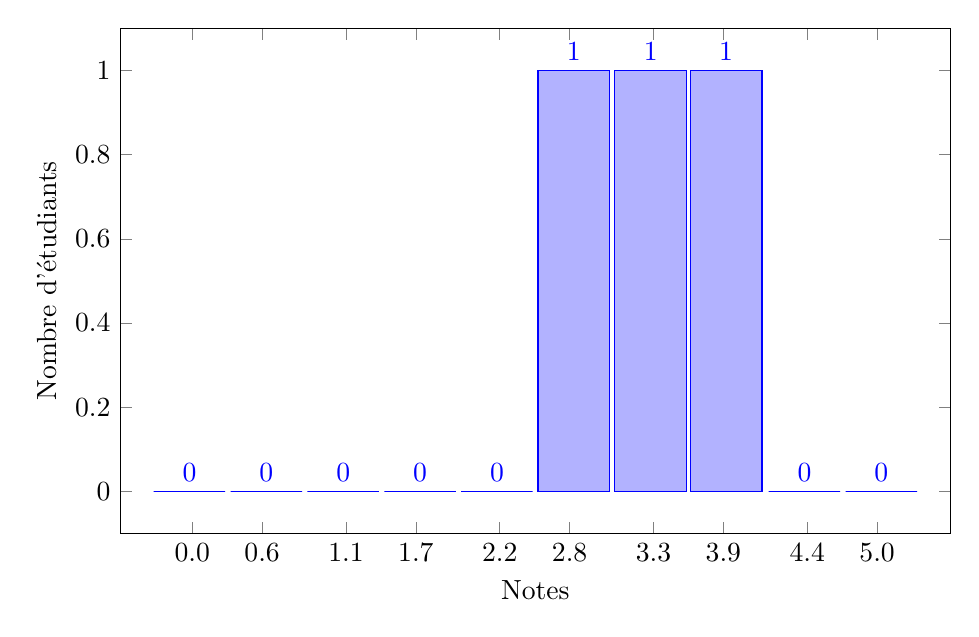
\begin{tikzpicture}
\begin{axis}[
width=\textwidth,
ybar=1.0,
bar width=0.9090909090909092cm,
height=8cm,
ylabel={Nombre d'étudiants},
xlabel={Notes},
xtick=data,
xtick align=inside,
xticklabel style={align=center},
xtick={0.3, 0.8, 1.4, 1.9, 2.5, 3.0, 3.6, 4.1, 4.7, 5.2},
xticklabels={0.0, 0.6, 1.1, 1.7, 2.2, 2.8, 3.3, 3.9, 4.4, 5.0, 5.5},
nodes near coords,
area style,
]
\addplot coordinates {
(0.28, 0) (0.83, 0) (1.38, 0) (1.93, 0) (2.48, 0) (3.03, 1) (3.58, 1) (4.12, 1) (4.68, 0) (5.23, 0) };
\end{axis}
\end{tikzpicture}
    \end{center}

    %%% fin - Répartition des résultats %%%

\subsection{Tableau d'analyse des résultats}

    %%% debut - Tableau des résultats %%%

    
    \begin{center}
        \begin{tabular}{|c|c|c|c|c|c|}
        \hline
        \bfseries Nom & \bfseries Prenom & \bfseries Total & \bfseries E1  & \bfseries E2  \\
        \hline

      \ \bfseries ageugeu & \bfseries beubeubeu & \num{3} & \num{1}& \num{2} \\
      \hline

      \ \bfseries joeystar & \bfseries Jonathan & \num{4} & \num{1}& \num{3} \\
      \hline

      \ \bfseries littlewood & \bfseries boumbazar & \num{3.5} & \num{1}& \num{2.5} \\
      \hline

\end{tabular}
\end{center}


    %%% fin - Tableau des résultats %%%
\newpage

\subsection{Compétences du devoir}

    %%% debut - tableau %%%
    
    \begin{center}
         -  \\
 C4C01 - Additions de nombres relatifs\\
C4G22 - Contraposée du théorème de Pythagore
    \end{center}

    %%% fin - tableau %%%

    
\subsection{Analyse par exercices}

    %%% debut - tableau %%%
    
    \begin{center}
        \begin{tabular}{|c|c|c|c|c|}
\hline
 & q1 & Moyenne & q3 & Barème \\ \hline
Exercice 1 & {\scriptsize 1{,}00} & $\mathbf{1{,}00}$ & {\scriptsize 1{,}00} & 1 \\ \hline
Exercice 2 & {\scriptsize 2{,}25} & $\mathbf{2{,}50}$ & {\scriptsize 2{,}75} & 4.5 \\ \hline
\end{tabular}
    \end{center}

    %%% fin - tableau %%%

\begin{multicols}{2}

    %%% debut - explications %%%
    \boite{Commentaires :}{
    
        %%% debut - analyse %%%

        \begin{itemize}
\item Exercices bien réussis : 2
\item Exercices très bien réussis : 1
\end{itemize}


        %%% fin - analyse %%%

        
        Note moyenne obtenue au contrôle : \begin{center} $\mathbf{3{,}5/5{,}5}$\end{center}
        Explications pour les exercices : 
        \begin{itemize}
            %\item Exercice 1 :\\ 
\item Exercice 2 :\\ Reprendre le cours sur cette compétence. Effectuer l'exercice sur une feuille en y inscrivant le numéro et la page d l'exercice. Remettre ce document au professeur pour correction.
        \end{itemize}
        

    }
    %%% fin - explications %%%
    
    \columnbreak

    %%% debut - radar %%%
    
    
\begin{center}
    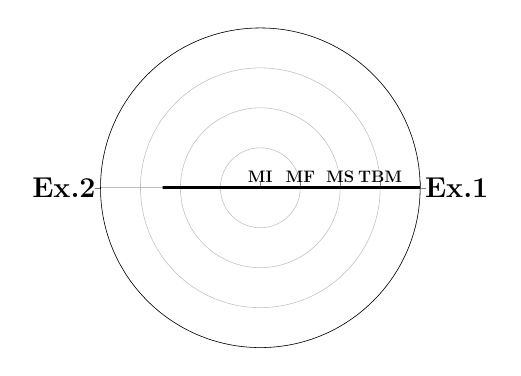
\begin{tikzpicture}[scale=0.5]
        \begin{polaraxis}[
            width=0.8\textwidth,
            xtick={0.0,180.0},
            xticklabels={\huge \bfseries Ex.1,\huge \bfseries Ex.2},
            ymin=0, ymax=100,
            ytick={0,25,50,75,100},
            yticklabels={\large \bfseries MI,\large \bfseries MF,\large \bfseries MS,\large \bfseries TBM, }
        ]
        \addplot+[mark=none,fill=blue,opacity=0.5] coordinates {
            (0.0,100.0)  (180.0,55.55555555555556)  
        } -- cycle;
        
        \addplot+[mark=none,fill=none,opacity=1,line width = 2pt,dashed,color=black] coordinates {
                    (0.0,100.0)  (180.0,50.0)  
                } -- cycle;
        
        \addplot+[mark=none,fill=none,opacity=1,line width = 2pt,dashed,color=black] coordinates {
                    (0.0,100.0)  (180.0,61.111111111111114)  
                } -- cycle;
        
        \end{polaraxis}
    \end{tikzpicture}
\end{center}


    %%% fin - radar %%%

\end{multicols}



                \newpage

                
\section{Résultats de AGEUGEU Beubeubeu}

    %%% debut - tableau %%%
    \boitesignature{
    \textbf{Contrôle effectué le : 15/10/2024} \\
    \textbf{Thèmes abordés : }Pythagore
    }{\begin{center}\bfseries\huge{3/5{,}5} \end{center}}

    \begin{center}
        
\begin{tabular}{|c|c|c|}
      \hline
       & \bfseries Exercice 1  & \bfseries Exercice 2  \\
      \hline
      \bfseries Points  & 1 & 2 \\
      \hline
      \bfseries Barème  & 1 & 4.5 \\
      \hline
\end{tabular}

    \end{center}

    %%% fin - tableau %%%

\begin{multicols}{2}

    %%% debut - explications %%%
    \boite{Commentaires :}{
        
            \begin{itemize}

                \item \textbf{Exercice 2} à retravailler.\\ 
                    Reprendre le cours sur cette compétence. Effectuer l'exercice sur une feuille en y inscrivant le numéro et la page d l'exercice. Remettre ce document au professeur pour correction.
                    
            
            \end{itemize}

    
    }
    %%% fin - explications %%%
    
    \columnbreak

    %%% debut - radar %%%
    
    
\begin{center}
    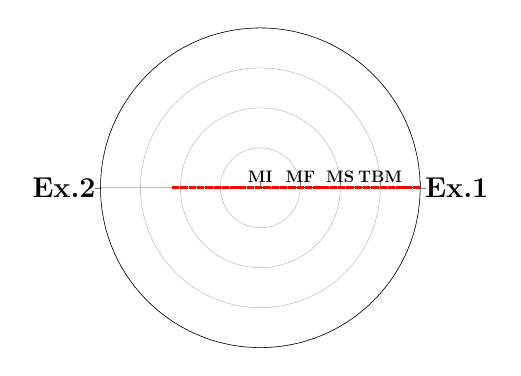
\begin{tikzpicture}[scale=0.5]
        \begin{polaraxis}[
            width=0.8\textwidth,
            xtick={0.0,180.0},
            xticklabels={\huge \bfseries Ex.1,\huge \bfseries Ex.2},
            ymin=0, ymax=100,
            ytick={0,25,50,75,100},
            yticklabels={\large \bfseries MI,\large \bfseries MF,\large \bfseries MS,\large \bfseries TBM, }
        ]
        \addplot+[mark=none,fill=blue,opacity=0.5] coordinates {
            (0.0,100.0)  (180.0,44.44444444444444)  
        } -- cycle;
        
        \addplot+[mark=none,fill=none,opacity=1,line width = 2pt,dashed,color=red] coordinates {
                    (0.0,100.0)  (180.0,55.55555555555556)  
                } -- cycle;
        
        \end{polaraxis}
    \end{tikzpicture}
\end{center}


    %%% fin - radar %%%

\end{multicols}

                \newpage
                
\section{Résultats de JOEYSTAR Jonathan}

    %%% debut - tableau %%%
    \boitesignature{
    \textbf{Contrôle effectué le : 15/10/2024} \\
    \textbf{Thèmes abordés : }Pythagore
    }{\begin{center}\bfseries\huge{4/5{,}5} \end{center}}

    \begin{center}
        
\begin{tabular}{|c|c|c|}
      \hline
       & \bfseries Exercice 1  & \bfseries Exercice 2  \\
      \hline
      \bfseries Points  & 1 & 3 \\
      \hline
      \bfseries Barème  & 1 & 4.5 \\
      \hline
\end{tabular}

    \end{center}

    %%% fin - tableau %%%

\begin{multicols}{2}

    %%% debut - explications %%%
    \boite{Commentaires :}{
        Les compétences semblent suffisamment maîtrisées, \textbf{bien joué} !
    }
    %%% fin - explications %%%
    
    \columnbreak

    %%% debut - radar %%%
    
    
\begin{center}
    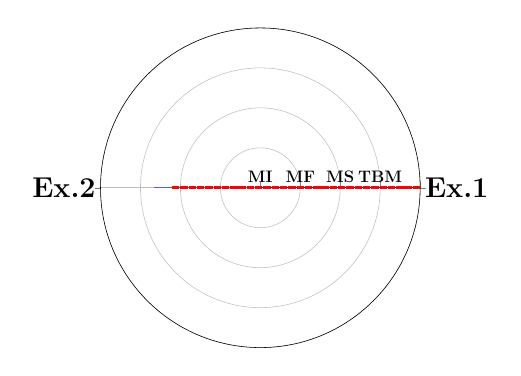
\begin{tikzpicture}[scale=0.5]
        \begin{polaraxis}[
            width=0.8\textwidth,
            xtick={0.0,180.0},
            xticklabels={\huge \bfseries Ex.1,\huge \bfseries Ex.2},
            ymin=0, ymax=100,
            ytick={0,25,50,75,100},
            yticklabels={\large \bfseries MI,\large \bfseries MF,\large \bfseries MS,\large \bfseries TBM, }
        ]
        \addplot+[mark=none,fill=blue,opacity=0.5] coordinates {
            (0.0,100.0)  (180.0,66.66666666666667)  
        } -- cycle;
        
        \addplot+[mark=none,fill=none,opacity=1,line width = 2pt,dashed,color=red] coordinates {
                    (0.0,100.0)  (180.0,55.55555555555556)  
                } -- cycle;
        
        \end{polaraxis}
    \end{tikzpicture}
\end{center}


    %%% fin - radar %%%

\end{multicols}

                \newpage
                
\section{Résultats de LITTLEWOOD Boumbazar}

    %%% debut - tableau %%%
    \boitesignature{
    \textbf{Contrôle effectué le : 15/10/2024} \\
    \textbf{Thèmes abordés : }Pythagore
    }{\begin{center}\bfseries\huge{3{,}5/5{,}5} \end{center}}

    \begin{center}
        
\begin{tabular}{|c|c|c|}
      \hline
       & \bfseries Exercice 1  & \bfseries Exercice 2  \\
      \hline
      \bfseries Points  & 1 & 2.5 \\
      \hline
      \bfseries Barème  & 1 & 4.5 \\
      \hline
\end{tabular}

    \end{center}

    %%% fin - tableau %%%

\begin{multicols}{2}

    %%% debut - explications %%%
    \boite{Commentaires :}{
        Les compétences semblent suffisamment maîtrisées, \textbf{bien joué} !
    }
    %%% fin - explications %%%
    
    \columnbreak

    %%% debut - radar %%%
    
    
\begin{center}
    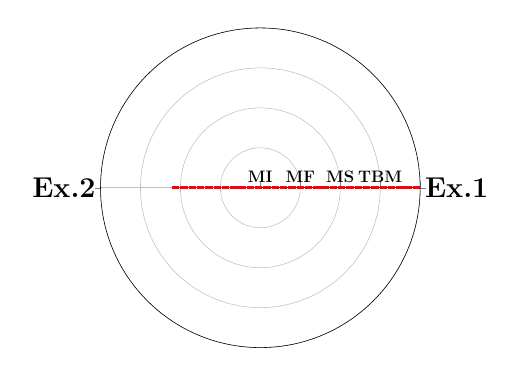
\begin{tikzpicture}[scale=0.5]
        \begin{polaraxis}[
            width=0.8\textwidth,
            xtick={0.0,180.0},
            xticklabels={\huge \bfseries Ex.1,\huge \bfseries Ex.2},
            ymin=0, ymax=100,
            ytick={0,25,50,75,100},
            yticklabels={\large \bfseries MI,\large \bfseries MF,\large \bfseries MS,\large \bfseries TBM, }
        ]
        \addplot+[mark=none,fill=blue,opacity=0.5] coordinates {
            (0.0,100.0)  (180.0,55.55555555555556)  
        } -- cycle;
        
        \addplot+[mark=none,fill=none,opacity=1,line width = 2pt,dashed,color=red] coordinates {
                    (0.0,100.0)  (180.0,55.55555555555556)  
                } -- cycle;
        
        \end{polaraxis}
    \end{tikzpicture}
\end{center}


    %%% fin - radar %%%

\end{multicols}

                \newpage
                
                \end{document}
            